\begin{abstract}
%%%%%%%%%%%%%%%%%%%
We demonstrate a system for direct authentication of users to their head--worn wearable device through a novel approach that identifies users based on motion signatures extracted from their head--movements. This approach is in contrast to existing indirect authentication solutions via smartphone or using touch--pad swipe patterns. The system, dubbed~\systemname, is a software authentication solution that leverages unique motion patterns created when users shake their head in response to music played on the head--worn device, and sensed through integrated accelerometers. In this demo, we demonstrate~\systemname~on Google GLASS and show the effectiveness of the system in two authentication modes, that include (i) a trained user reliably authenticated to the owned GLASS device, and (ii) an attacker being prevented from login when attempting to login to the GLASS device by imitating the owner's head--movements. 
\iffalse
In this project, we demonstrate a practical novel approach to authenticate a user on a head-worn device with limited input hardware, by monitoring the user's unique head movement patterns stimulated by an external audio music. Existing solutions today rely on indirect authentication via smartphone or swipe pattern on the built-in touchpad. These could be cumbersome and vulnerable. In the other hand, biometric approach such as fingerprint and iris are subject to the availability of the sensor unit. The proposed system, ~\systemname, addresses these concerns, and provide a practical solution with high authentication accuracy. In average, our system can achieve true acceptance rate of 95.57\% while the false acceptance rate is only 4.43\%.
\fi
\end{abstract}

\section{Introduction}

Wearable devices are increasingly becoming an integral part of the pervasive sensing and computing infrastructure today. These devices often collect data about users, which are also frequently shared to the users' multiple devices; for example, as background notifications. In such a wireless network of human sensing wearable devices the concerns of owner's privacy and security from malicious users are paramount, thus calling for an effective and robust user--authentication solution for wearable devices. Prior works have explored this problem in point--specific applications for limiting privacy threats~\cite{hoyle2015sensitive,hoyle2014privacy,jana2013scanner}, for example from photography--enabled wearable devices. In addition, existing approaches for authentication on wearables are limited to an indirect method -- channeling through a smartphone~\cite{pebble} or using swipe patterns integrated touch--pads~\cite{googleglass}. Such approaches impose a requirement for the user to carry both device, smartphone and the wearable all the time, and also have an increased chance of being compromised if either of the devices are lost or stolen.
Therefore, a direct, secure and robust authentication solution for wearable devices is the need of the day.

In this work, we propose a novel approach for direct authentication on wearable devices through signatures generated from the device user's motion patterns. In particular, we design a system,~\systemname, for head--worn wearable devices, that identifies users based on their head--movement patterns. We design a software system, in the form of an authentication service on a head--worn wearable device, that authenticates users to their device by recognizing their unique head--movement signatures. This approach is in contrast and more secure than linking the wearable device to user's email~\cite{googleglass} and other online accounts~\cite{fitbit}. In this work, we demonstrate~\systemname through an authentication service implementation on Google GLASS and show its reliability to user--authentication and robustness to imitation attacks from adversaries. In Fig.~\ref{fig:headbanger-illustrate} we illustrate the two modes of authentication, using~\systemname, that we have implemented and will demonstrate.

In the following sections we will describe the~\systemname system design briefly in Section~\ref{sec:system}, we refer the reader to our full paper in PerCom 2016 for more details on the system design and evaluations. Section~\ref{sec:demo}describes the implementation and demonstration plans.

\begin{figure}
	%\begin{subfigure}
	\centering
	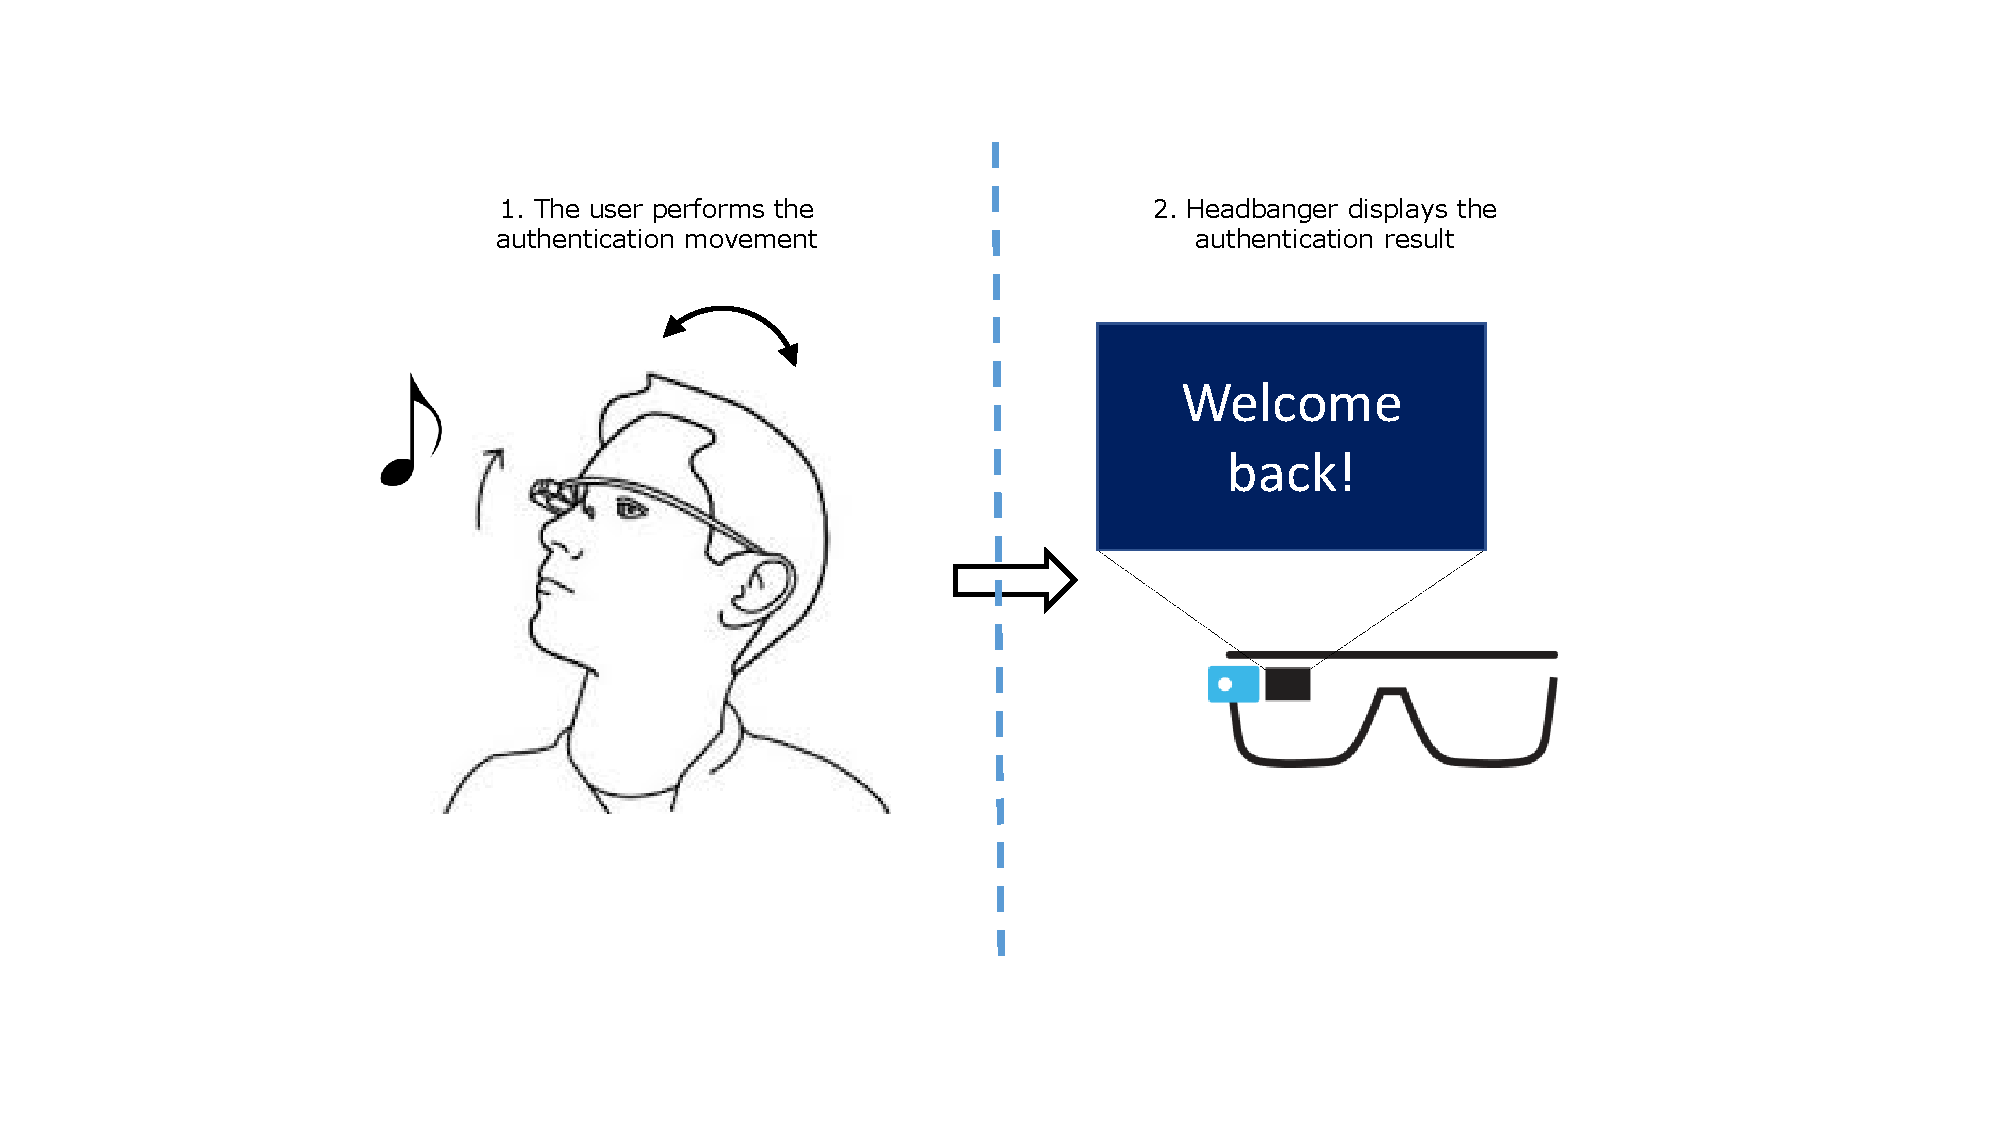
\includegraphics [width=0.9\columnwidth]{pic/demo_illus2.pdf}\\
	\centering
	(a)\\

	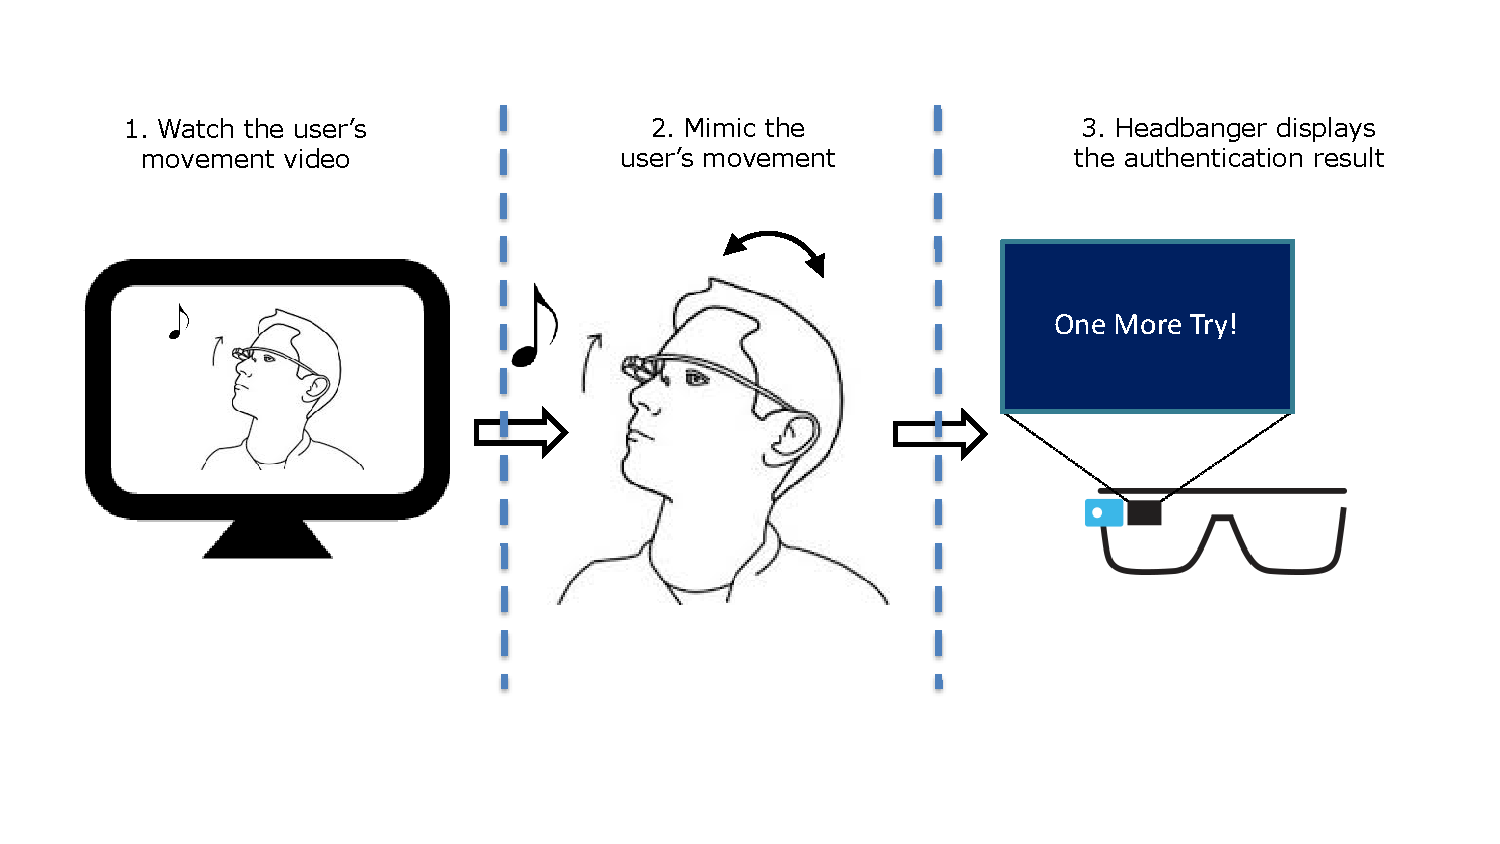
\includegraphics [width=0.9\columnwidth]{pic/demo_illus.pdf}\\
	\centering
	(b)\\
	%\end{subfigure}

\caption{Illustration of Headbanger demo when (a) authenticating owner for login, (b) preventing an attacker from login.}
\label{fig:headbanger-illustrate}
\end{figure}

\iffalse
After decades of effort on hardware and battery research, wearable devices become pervasive and an integral part of humans lives~\cite{googleglass,smartwatch,fitbit}. The devices often collect data about user's activity status and his surroundings. At the same time, some wearable device are even able to forward notification to the user for the background service. The security and  privacy protection for both collected data and background notification become critically important. There have been works ~\cite{hoyle2015sensitive,hoyle2014privacy,jana2013scanner} on limiting privacy  threats from ubiquitous photography enabled by the wearable devices, robust usable and secure authentication systems leveraging the devices have not emerged.  The authentication system for these device has to strike for a appropriate balance of user convenience, energy efficient, and low cost.

Authentication on most of today's commercialized wearable device relies on indirect method, where users needs to log into their wearable devices via smartphones. This mechanism  , however, impose an requirement that the devices have to be paired and accompanied by smartphones, which can be highly inconvenient in reality. The security of this approach is also in question as it increases the chance of hacking into both devices if either is lost or stolen. Some devices including Google Glass~\cite{googleglass} and FitBit's health tracker~\cite{fitbit} allow linking the device to online accounts instead of a mobile device for convenience,  which, however, does not add to security.
\fi

